\documentclass{templatearticle}
\usepackage{multicol}
\usepackage{multirow}
\usepackage[cols=3,style=long]{glossary}
\usepackage[geometry]{ifsym}

% -----------------------------------------------------------------------------
% User settings
% -----------------------------------------------------------------------------
\myDoctype {Projektspezifikation}
\myDivision {}
\myTitle {Cube Circle Tower Defense (CCTD)}
\mySubTitle {}
\myAuthor {Rolf Koch, Lukas Spirig, Benjamin Felder, Fabian Eriksson, Nathanael Koch}
%\myCompany {}
%\myStreet {}
%\myPLZ {}
%\myTown {}
%\myPhone {}
%\myFax {}
%\myWebsite {}
\myVersion {1.0}
%\myConfidential{Vertraulich}
%\myDraft{Entwurf}
\myLanguage{german} % german or english
\makeglossary 		% Setup Glossary

% -----------------------------------------------------------------------------
% Document: provide the two files abstract.tex and history.tex
% -----------------------------------------------------------------------------
\begin{document}
\setupLanguage            % setup configured language
\setupWatermarks          % setup watermarks
\printTitlePage{abstract} % include "abstract.tex"
\printLeader{history}     % include "history.tex"

% -----------------------------------------------------------------------------
% Glossary: Default Set of Glossary Entries. More can be added 
%               anywhere in the Document.
% -----------------------------------------------------------------------------

\setlength{\descriptionwidth}{0.75\linewidth}
\glossary{name={CCTD}, description={Cube Circle Tower Defense}}{CCTD}

% -----------------------------------------------------------------------------
% Input user files with LaTex text sections
% -----------------------------------------------------------------------------
\section{Projekt Management} \label{sec:Projekt-Management}
\subsection{Aktueller Status} \label{sec:Aktueller-Status}
In dieser Sektion befindet sich ein Vergleich des geplanten Aufwands und des tatsächlich erreichten Resultats sowie dessen jeweiliger Aufwand der für die einzelnen Tasks geleistet wurde.

\begin{table}[htp]
\begin{tabular}{ | p{6.5cm} | l  | l | l | l |}
\hline
\textbf{Aufwände} & \textbf{Aufw. Geplant}  & \textbf{Aufw.} & \textbf{Aufw. p.P} & \textbf{Anz. P} \\ \hline \hline
Spielprinzip definiert & ? 0  & 15 & 3 & 5 \\ \hline
Entwicklungs Umgebung definiert & ?  & 6 & 3 & 2 \\ \hline
\textbf{Projekt Skizze:}
\begin{itemize}
\item Projekt Idee
\item Hauptanwendungsfall
\item Weitere Anforderungen
\item Ressourcen
\item Risiken
\item Grobplanung
\item Kundennutzen
\item Wirtschaftlichkeit 
\end{itemize}& ?   & 40 & 8 & 5 \\ \hline
\textbf{Präsentation Projekt Skizze} & ?  & 5 & 5 & 1 \\ \hline
Applikations Grundgerüst erstellt & 5  & \textcolor{red}{nicht erfüllt} & ? & ? \\ \hline
Anwendungsfälle detailiert ausformuliert & 8  & \textcolor{red}{12} & 6 & 2 \\ \hline
Domänenmodel Entwurf & 10 & 10 & 2 & 5 \\ \hline
Projekt Management auf neusten Stand gebracht  & 7 & 7 & 7 & 1 \\ \hline
Architektur & 5 & 5 & 5 & 1 \\ \hline
Supplementary Specification erstellt & 6  & 6 & 6 & 1 \\ \hline
System Sequenzdiagram & 8  & 8 & 8 & 1 \\ \hline
Glossar erstellt & 3  & \textcolor{red}{6} & 2 & 3 \\ \hline
Vision fertig gestellt & 4 & 3 & 3 & 1 \\ \hline
Domänenmodell erstellt & 5  & 5 & 5 & 1 \\ \hline
Java Tests bezüglich Client / Server verhalten & 12 & \textcolor{red}{nicht erfüllt} & ? & ? \\ \hline
Welche Daten werden übertragen & 3 & \textcolor{red}{nicht erfüllt} & ? & ? \\ \hline
\textbf{Analyse Dokumentation fertigstellen} & 5 & 5 & 5 & 1 \\ \hline
\textbf{Analyse Präsentation erstellt} & 3 & 3 & 3 & 1 \\ \hline
UML Klassendiagram Entwurf & 3 & 3 & 1.5 & 2 \\ \hline
\end{tabular}
\caption{Projekt Management: Aktueller Status}
\end{table}

\subsection{Massnahmen} \label{sec:Massnahmen}
Für die Design Phase wird nun vermehrt auch erster Javacode generiert. In der Iteration 3 (Analyse + Design) 
wird nun auch das Applikations Grundgerüst erstellt und erste Java Tests bezüglich Client / Server verhalten durchgeführt. Die Tasks wurden verschoben.

\subsection{Weitere Planung} \label{sec:Weitere-Planung}

\textbf{Analyse + Design (Iteration 3)}

Wir befinden uns momentan in dieser Iteration 3 und somit in der Elaborations Phase. Zu diesem Zeitpunkt geht die Analyse Phase in die Design Phase über.

\begin{table}[htp]
\begin{tabular}{ | l | l | l |  p{6.5cm} | l |}
\hline
Phase & Woche & Iteration & Task & Geplanter Aufwand \\ \hline \hline
Elaboration & 42 &  3  & Use Cases fertig & 4 \\ \hline
 &  &  & Supplementary Specification fertig falls benötigt & 3 \\ \hline
 &  &  & System-Sequenzdiagram erstellt & 3 \\ \hline
 &  &  & Glossar erstellt & 3 \\ \hline
 &  &  & Vision fertig & 4 \\ \hline
 &  &  & Domänenmodell erstellt & 3 \\ \hline
 &  &  & Erste Java Tests bezüglich Client / Server verhalten & 12 \\ \hline
 &  &  & welche Daten werden übertragen & 6 \\ \hline
 &  &  & Applikations Grundgerüst erstellt & 5 \\ \hline
 \hline
 & 43 &  & \textcolor{red}{Abgabe Analyse} & 5 \\ \hline
 &  &  & \textcolor{red}{Präsentation Analyse} & 1 \\ \hline
 &  &  & erste Version UML Klassendiagram & 15  \\ \hline
 &  &  & erste Version Architekturdokumente & 12  \\ \hline
\end{tabular}
\caption{Projekt Management: Iteration 3}
\end{table}
Woche 42: 40 Stunden. Pro Person: 8 Stunden

Woche 43: 33 Stunden. Pro Person: 6,6 Stunden

Total: 73 Stunden. Pro Person: 14,6 Stunden

\textbf{Design (Iteration 4)}

Ab Woche 44 startet die Design Phase mit der Iteration 4 bei der es hauptsächlich um das Code Design geht.

\begin{table}[htp]
\begin{tabular}{ | l | l | l |  p{6.5cm} | l |}
\hline
Phase & Woche & Iteration & Task & Geplanter Aufwand \\ \hline
\hline
Construction & 44 &  4  & UML Klassendiagram & 10 \\ \hline
 &  &  & UML Interaktionsdiagram für ausgewählte Systemoperationen & 10 \\ \hline
 &  &  & Architekturdokumente fertig 5 \\ \hline
 &  &  & Implementation des UML Klassendiagrams in Java & 15 \\ \hline
 &  &  & Test der Zusammenhänge: ev. Klassendiagram überarbeiten & 5 \\ \hline \hline
 & 45 &  & UML Klassendiagram & 15 \\ \hline
 &  &  & UML Interaktionsdiagram für ausgewählte Systemoperationen & 10 \\ \hline
 &  &  & Architekturdokumente fertig & 5 \\ \hline
 &  &  & Design Präsentation fertig & 5 \\ \hline
 &  &  & Erste Implementation der Klassen inklusive Methoden und Eigenschaften &  15 \\ \hline
\end{tabular}
\caption{Projekt Management: Iteration 4}
\end{table}

Woche 44: 45 Stunden. Pro Person: 9 Stunden

Woche 45: 50 Stunden. Pro Person: 10 Stunden

Total: 95 Stunden. Pro Person: 19 Stunden

\subsection{Anpassung der Projekt Aufwand Schätzung} \label{sec:Anpassung-der-Projekt-Aufwand-Schaetzung}

Aufgrund der nun vorliegenden Zahlen muss die eher etwas übertriebene Aufwandschätzung korrigiert werden. Geschätzt war ursprünglich ein Aufwand von 600 Mannstunden verteilt auf 5 Personen. Aktuelle Zahlen zeigen, dass dieser Aufwand voraussichtlich nicht benötigt wird.

Wir setzen daher den geschätzten Aufwand neu auf ca 450 Stunden fest. Dies entspricht etwa einem Aufwand von 90 Stunden pro Iteration Total $\rightarrow$ 45 Stunden pro Woche Total $\rightarrow$ 9 Stunden pro Person pro Woche.

\subsection{Risiken} \label{sec:Risiken}
\subsubsection{Nachfrage} \label{subsec:Risiken-Nachfrage}
Nach einer kurzen Suche mit Google ergeben sich etliche Treffer für ``Tower Defense``-Spiele in etlichen Formen. Zum Beispiel towerdefence.net listet 196 unterschiedliche ``Tower Defense``-Implementationen (Stand: 01.10.2010). Ausserdem unterstützen mehrere Multiplayer Strategy Spiele einen Tower Defense Modus (Warcraft 3, Starcraft 2, ...). \\
Ein weiteres Problem stellt die Gewinngenerierung dar. Die meisten ``Tower Defense``-Spiele sind entweder eine Erweiterung zu einem bereits existierenden Spiel oder können Gratis heruntergeladen werden.

\subsubsection{Projektumfang} \label{subsec:Risiken-Projektumfang}
Der Projektumfang ist für die kurze Zeit von einem Semester gross gehalten. Deswegen kann es schwierig werden das ganze Produkt mit allen vorgesehenen Features in der kurzen Zeit zu implementieren. \\
Stellt sich im Verlaufe des Projektes heraus, dass das Projekt nicht im gegebenen Zeitrahmen zum vollständigen Abschluss gebracht werden kann, werden gewisse Features weggelassen.

\subsubsection{Mitarbeiter Motivation} \label{subsec:Mitarbeiter-Motivation}
Da das Projekt `nur' auf Basis eines Wahlmoduls entwickelt wird und keine reale Bezahlung stattfindet, kann es passieren, dass sich einzelne Mitarbeiter des Teams nicht motivieren können für das Projekt zu arbeiten. \\
Dies kann eventuell dazu führen, dass nicht alle geplanten Tasks durchgeführt werden und Tasks immer weiter nach hinten geschoben werden, was schlussendlich zum Risiko `Projektumfang' führt und eine Reduktion der Features getätigt werden muss um das Projekt doch noch vollständig abschliessen zu können.

 \newpage
\section{Anwendungsfälle}

\subsection{Use Case Diagram}

\begin{figure}[htb]
 \begin{center}
  \leavevmode
  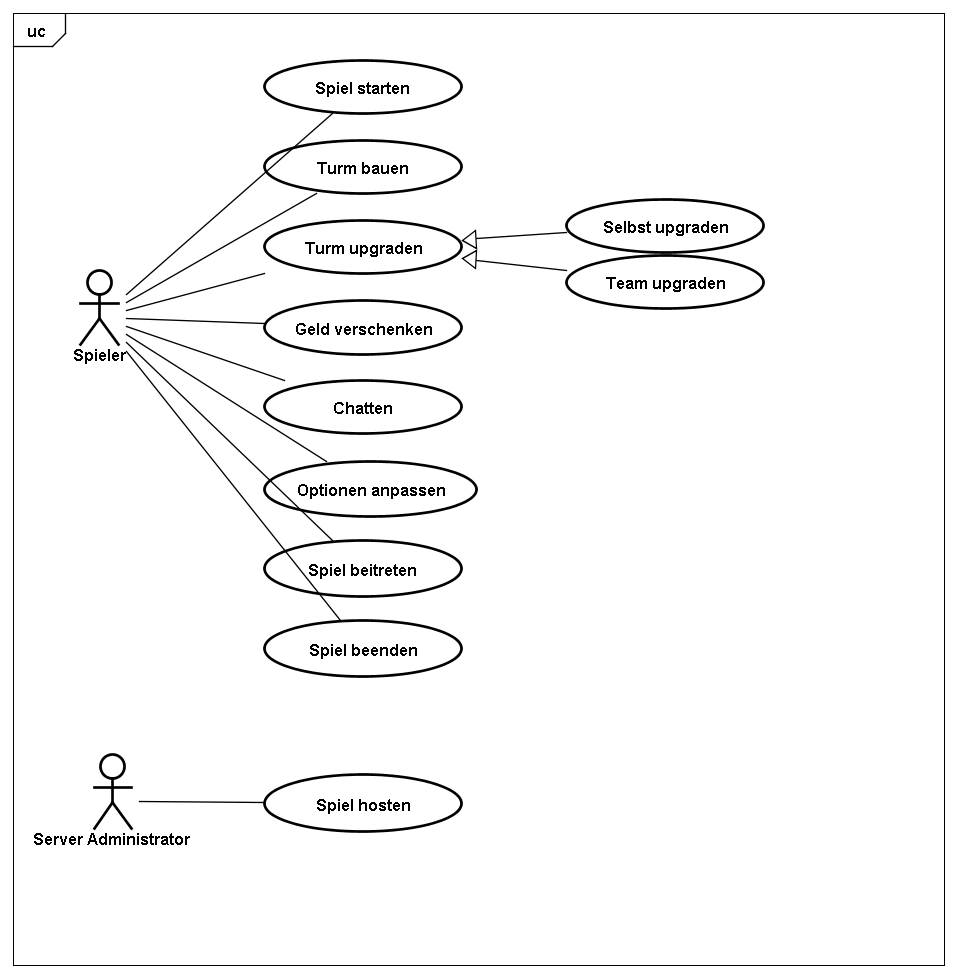
\includegraphics[width=0.95\textwidth]{usecasediagram.png}
 \end{center}
 \caption{Use Case-/Anwendungsfall-Diagram}
 \label{fig:usecasediagram}
\end{figure}

Es existieren zwei Hauptaktoren. Ein Spieler und ein Server Administrator. Total können maximal vier Spieler an einem Spiel teilnehmen. Pro Spiel benötigt es mindestens einen Server Administrator. Der Server Administrator zählt gleichzeitig auch als Spieler. Für ein Einzelspieler Spiel muss braucht es also einen Server Administrator der gleichzeitig auch als Spieler fungiert. Für Multiplayer Spiele können dann jedoch noch bis zu drei zusätzliche Spielern beitreten nebst dem Server Administrator.

Wir haben als Haupt Use Case `Spiel starten' ausgewählt. Als Casual haben wir `Spiel hosten', `\glossary{name={Turm}, description={Eine Einheit, die vom Benutzer gebaut wird und autonom auf Creeps schiesst.}}{Turm} bauen' und `Turm upgraden' ausgewählt. Als Brief stehen somit noch `Spiel beitreten', `Geld verschenken', `Chatten', `Optionen anpassen', `Spiel beenden' und die beiden Upgrade Funktionalitäten `Selbst upgraden' und `Team upgraden' zur Verfügung. Diese beiden Upgrade Funktionalitäten stellen zwei Ausprägungen des `Turm upgraden' dar, da sie unterschiedlich funktionieren, je nach dem ob man einen eigenen Turm oder den Turm eines Kollegen upgraden möchte.

\subsection{Use Case UC1: Spiel starten}

\textbf{Primary Actor:} Spieler

\textbf{Stakeholder and Interests:}

\begin{itemize}
\item Spieler: Möchte so schnell wie möglich ein Spiel starten und keine grosse Verzögerung durch die Authentifizierung
\item Server: Möchte die Verbindungen verwalten
\end{itemize}

\textbf{Precondition:}
\begin{itemize}
\item Der Spieler möchte ein Spiel starten 
\item Es muss ein Server aktiv sein
\end{itemize}


\textbf{Postcondition:}
\begin{itemize}
\item Programm ist offen und eine Verbindung steht
\end{itemize}


\textbf{Main Success Scenario:}

\begin{enumerate}
\item Spieler startet Programm
\item Programmfenster erscheint
\item Spieler gibt, falls nicht gespeichert, Spielername ein 
\item Spieler wählt Einzelspiel oder Multiplayer

\begin{enumerate}
\item Spieler wählt Einzelspiel

\begin{enumerate}
\item Programm startet ein Einzelspiel
\item Programm verwaltet Spiel
\end{enumerate}

\item Spieler wählt Multiplayer
\begin{enumerate}
\item Spieler kann wählen, ob er ein Spiel hosten möchte (UC2) oder einem Spiel beitreten möchte (UC3)
\item Spieler wartet dann in der Lobby, bis genügend andere Spieler anwesend sind
\end{enumerate}

\end{enumerate}

\end{enumerate}


\textbf{Extensions:}
\begin{itemize}
\item Wenn während eines Multiplayer Matches das Programm abstürzt oder die Verbindung verloren geht, soll der Server das erkennen und entsprechend reagieren.
\item Wenn der Spielerhost die Verbindung verliert, bricht das Spiel ab.
\end{itemize}

\textbf{Special Requirements:}

Die Fenstergrösse des Programms soll variabel sein


\textbf{Technology and Data Variations List:}

-


\textbf{Frequency of Occurrence:}

Zu Beginn


\textbf{Open Issues:}

-





\subsection{Use Case UC2: Spiel hosten}

\textbf{Primary Actor:} Server Administrator

Ein Spieler startet einen Spiel-Server auf den sich die Clients einloggen können.

Der Server überprüft den Spielername und verwaltet alle aktiven Verbindungen. Wenn alle Spieler bereit sind, wird das Spiel gestartet.

\glossary{name={Wave}, description={(Welle), besteht aus einer variirenden Anzahl an Creeps, die zusammen auf das Spielfeld tretten}}{Wave}
Der hostende Client übernimmt dann das Wave-Handling und das Creep-Handling.

Wenn eine Verbindung zu einem Spieler verloren geht, informiert er die anderen Spieler.

\glossary{name={Spawn-Point}, description={Sind die Punkte auf der Karte, wo die Creeps auf das Spielfeld tretten}}{Spawn-Point}
Wenn ein Spieler seine Verbindung trennt, entfernt er die Türme des entsprechenden Spielers und auch den zugehörigen Wave-Spawn-Punkt.




\subsection{Use Case U3: Spiel beitreten}
\textit{Brief}

\textbf{Primary Actor:} Spieler

Ein Spieler kann einem Match beitreten. Dies kann er über die Adresse tun.




\subsection{Use Case UC4: Turm bauen}

\textbf{Primary Actor:} Spieler

Das Spielfeld muss zusammengestellt werden. Das Spielfeld besteht aus einer (oder mehreren) Hintergrundgrafik, 
begrenzte Bauflächen, Spawn-Punkte für die Creeps, eine Route für die Creeps, Spielinfozeile und einem Baumenü.

Die Creeps müssen dynamisch über das Spielfeld bewegt werden und bei Tod entfernt werden.

Das Programm stellt anhand der Fenstergrösse einen Ausschnitt des Spielfelds dar. 

Der Spieler kann mit vordefinierten Tasten durch das effektive Spielfeld scrollen oder mit der 
Maus an einen entsprechenden Rand fahren, damit sich das sichtbare Spielfeld verschiebt.
Wichtig dabei ist, dass die Geschwindigkeit angepasst ist, damit eine Feinkontrolle möglich ist.

Der Spieler soll dann aus einer Liste von Türmen auswählen können und einen Turm per Drag-and-Drop auf dem 
Spielfeld platzieren können.

Ein Turm kann nur in der eigenen Baufläche platziert werden und darf nicht mit anderen Türmen überlappen. 

Wenn man einen Turm ``dragt'', soll die, für den Turm benötigte, Fläche unter dem Cursor angezeigt werden.

Daraus soll auch ersichtlich sein, ob der vorgesehene Bauplatz für den selektierten Turm auch gültig ist.

Wenn der Turm erfolgreich platziert wurde, soll er nach einer kurzen Konstruktionszeit aktiv werden.

%%% Hat nichts mit dem bauen des Turmes zu tun:
%Die Türme sollen eigenständig auf einen, nach Vorgaben ermittelten, Gegner schiessen.

%Bis ein Schuss den entsprechenden Gegner erreicht, dauert es einen kurzen Augenblick und erst beim effektiven 
%Treffer wird der Schaden verursacht, sei dies nun Einzel- oder Flächenschaden.




\subsection{Use Case UC5: Turm upgraden}

\textbf{Primary Actor:} Spieler

Der Prozess des Upgraden läuft wie folgt ab:

\begin{enumerate}
\item Der Spieler klickt auf den \glossary{name={Tower}, description={Siehe Turm}}{Tower}, den er gerne upgraden möchte
\item In der Übersichtsliste erscheint eine Liste von möglichen Upgrades und die Option den Turm wieder zu verkaufen
\item Nachdem ein Upgrade ausgewählt wurde, wird der Tower upgegradet, sofern genug Ressourcen zur Verfügung stehen
\item Der Tower ist deaktiviert, bis das Upgrade abgeschlossen ist.
\item Sobald das Upgrad fertig gestellt ist, fängt der Tower wieder an zu schiessen und ist entsprechend der Art des Towers und des Upgrades verbessert
\end{enumerate}




\subsection{Use Case UC6: Turm upgraden: Selbst upgraden}
\textit{Brief}

\textbf{Primary Actor:} Spieler

Ein Spieler kann seine Türme upgraden. Dieses Upgrad ist eindimensional und erhöht die Effizienz des primären Merkmals des Towers.




\subsection{Use Case UC7: Turm upgraden: Team upgraden}
\textit{Brief}

\textbf{Primary Actor:} Spieler

Einem Spieler wird bei Spielbeginn zufällig ein Attribut zugewiesen. (Splash, Speed, Range, Slow, Poison)
Er kann einen Tower eines andere Spieler upgraden und diesem Tower zusätzlich zu dessen Merkmal das Attribut hinzufügen, das der Spieler besitzt. 





\subsection{Use Case UC8: Geld verschenken}
\textit{Brief}

\textbf{Primary Actor:} Spieler

Ein Spieler kann einem anderen Spieler Ressourcen schicken. Er kann dabei frei den Spieler und die Ressourcenanzahl wählen.




\subsection{Use Case UC9: Chatten}
\textit{Brief}

\textbf{Primary Actor:} Spieler

Die Spieler sollen untereinander chatten können. Sowohl in der Lobby als auch im Spiel.
Durch drücken einer bestimmten Taste soll eine Eingabezeile erscheinen, in welche der Spieler eine 
Nachricht schreiben kann. Wenn die Nachricht mit Enter bestätigt wird, wird diese in einer Scroll-Liste
angezeigt, wobei die neuste Nachricht immer unten ist und der Scroll-Balken sich bei einer neuen Nachricht
automatisch nach unten verschiebt.
Bei jeder Nachricht wird auf der linken Seite der Spielername des Authors angegeben, damit auch klar ist,
von wem die Nachricht stammt. 



\subsection{Use Case UC10: Optionen anpassen}
\textit{Brief}

\textbf{Primary Actor:} Spieler

Der Spieler kann diverse Einstellungen anpassen.



\subsection{Use Case UC11: Spiel beenden}
\textit{Brief}

\textbf{Primary Actor:} Spieler

Der Spieler kann jederzeit das Spiel beenden. Dabei werden alle allfälligen Verbindungen getrennt.


 \newpage
\section{Zusätzliche Spezifikationen} \label{sec:Zusaetzliche-Spezifikationen}
\subsection{Einführung}
Diese Sektion beschreibt CCTD Spiel Anforderungen, die nicht in den Use Cases erfasst sind.
\subsection{Funktionalität}
\textbf{Protokollierung und Fehlerhandhabung}

Alle Fehler in einem persistenten Speicher protokollieren.

% \textbf{Sicherheit}
% 
% Um Spieler eindeutig zu identifizieren muss sich jeder Spieler einen Benutzer Namen anlegen. Über diesen Benutzernamen wird der Spieler dann als eindeutiger Spieler behandelt.

\subsection{Usability}
\textbf{Real Time Spielgeschehen}

Das Spiel soll sich als Echtzeit Spiel anfühlen. Das bedeutet jeder Command wird sofort und ohne grosse Zeitverzögerung ausgeführt und Spiel Elemente können auch ihrerseits jederzeit Aktionen ausführen ohne, dass der Spieler etwas dafür tut. z.B: Türme Schiessen, Creeps bewegen sich. 

\textbf{Spieler Focus}

Jeder Spieler ist für seine Ecke des Spielfeldes verantwortlich. Ein Spieler kann das Spielfeld jedoch erkunden und so zu seinen Kollegen schauen. Dies muss flüssig und vorallem schnell möglich sein, da er nicht viel Zeit hat um sich umzusehen ohne seine Türme zu stark zu vernachlässigen. Es sollte sehr rasch möglich sein für einen Spieler sich auf dem Spielfeld zu orientieren. Hierzu sollten Tastenkürzel bereitstehen um direkt von Basis zu Basis der Kollegen zu wechseln und auch ein Tastenkürzel um wieder zurück zur eigenen Basis zu wechseln.

Generell sollte es dem Spieler jedoch überlassen werden, wo er hinschauen möchte. Er sollte nicht gezwungen sein ständig auf einen Punkt zu starren.

\textbf{Informationen zu Spielelementen}

Ein Spieler sollte alle Spielelemente anklicken können. Hat er ein Element ausgewählt, werden ihm zusätzliche Informationen zu dem Element präsentiert. So kann er beispielsweise Türme seiner Kollegen anschauen und untersuchen oder Creeps anschauen, um festzustellen wie stark sie sind.

%\subsection{Spiel Integrität}
%Es muss viel Wert darauf gelegt werden, dass das Spielgeschehen ständig auf seine Integrität geprüft wird von allen Clienten. Jeder Client hat die Möglichkeit zum einen die Aktionen seines eigenen Spielers zu prüfen, um falsche Aktionen gar nicht erst zuzulassen. Zusätzlich kann jeder Client jedoch auch die Aktionen anderer Spieler prüfen.
%
%Besteht aus irgend einem Grund ein Integritäts Problem bei den Aktionen des lokalen Spielers so sind diese falschen Aktionen durch das Programm zu verhindern und dürfen nicht an den Server weitergeleitet werden. Das Spiel geht aber weiter.
%
%Besteht aus irgend einem Grund ein Integritäts Problem innerhalb des Spiels welches auf dem verhalten anderer Spieler basiert, so ist das Spiel auf der Stelle abzubrechen, da ein Spieler vermutlich zu bescheissen versucht. (Cheating)
%
\subsection{Wartbarkeit}

\textbf{Anpassbarkeit}

Das Spiel sollte schnell und einfach erweiterbar sein. Es sollen neue Creeps eingefügt werden können, neue Tower Modelle sollen erstellt werden können und neue Tower Updates sollten einfach hinzugefügt werden können.

\textbf{Konfigurierbarkeit}

Alle Einstellungen die man im Spiel vornehmen kann sollten in einem Config File gespeichert werden und sollten auch dort änderbar sein.
\subsection{Implementierungsbedingungen}
Das CCTD Spiel wird in Java entwickelt werden, da diese Programmiersprache von allen beteiligten beherrscht wird.
\subsection{kostenlose Open-Source-Komponenten}
Im Allgemeinen setzen wir auf möglichst viele kostenlose Java-basierte \glossary{name={Open-Source}, description={bedeutet, dass eine Software nach einem Prinzip der Offenheit entwickelt wurde. Sie wird dann meist mit einer Lizenz versehen, die die weiterverwendbarkeit der Software relativ detailiert regelt.}}{Open-Source}-Komponenten.

Folgende Komponenten werden mit hoher Wahrscheinlichkeit für das Spiel oder zu dessen Entwicklung verwendet:
\begin{itemize}
\item JUnit (Testing Framework)
\item Easymock (Testing Component)
\item Cobertura (Test Coverage Utility)
\item log4j (Protokollierungs Framework)
\end{itemize}
\subsection{Interfaces}
\textbf{Grundsätzliche Design Entscheidung:}

Das CCTD Spiel wird grundsätzlich für Computer Bildschirme (12''  und grösser mit einer Mindestauflösung von 1024x768) entwickelt.
Das Spiel wird auf eine Maus und Tastatur Bedienung ausgelegt.

\textbf{Erweiterbarkeit für spätere Releases:}

Das Spiel kann erweitert werden auf Touchscreen Bedienung und kleinere Bildschirme wie IPads oder Smartphones. 

Dies geschieht jedoch nicht im Release 1.
\subsection{Softwareschnittstellen}
Geplant sind keine speziellen Softwareschnittstellen.
\subsection{Rechtlich}

\textbf{Lizenzen}

Da unsere Software auch wieder als Open-Source publiziert wird ist es möglich andere Open-Source Software komponenten die unter den unten genannten Lizenzen veröffentlicht sind (aber nicht nur) zu verwenden. 

\begin{itemize}
\item Apache License, 2.0
\item BSD licenses (New and Simplified)
\item GNU General Public License (GPL)
\item GNU Library or "Lesser" General Public License (LGPL)
\item MIT license
\item Mozilla Public License 1.1 (MPL)
\item Common Development and Distribution License
\item Eclipse Public License
\item Creative Commons Attribution 2.5 License
\item Public Domain
\end{itemize}

Für mehr details besuchen sie bitte diese Seite: \url{http://en.wikipedia.org/wiki/Comparison_of_free_software_licenses}
 \newpage
\section{Diagramme}

\subsection{Domänenmodell}
Dieses Diagramm beschreibt das Problem (Die Umsetzung des Spiel), das gelöst werden muss.

\begin{figure}[htb]
 \begin{center}
  \leavevmode
  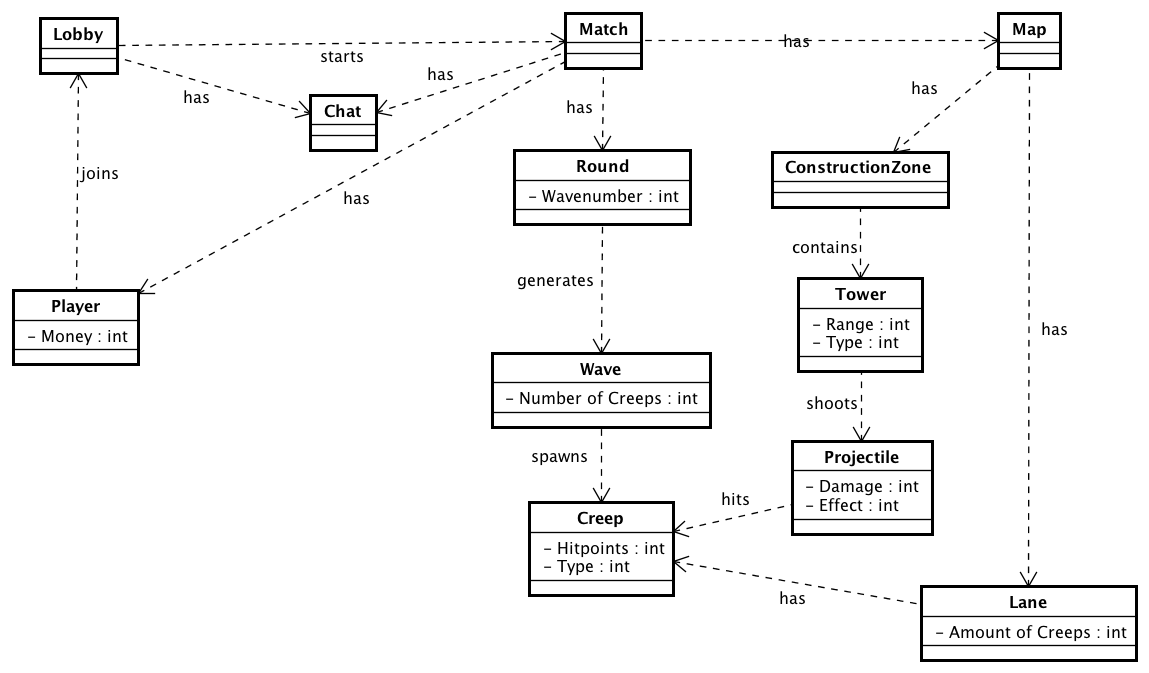
\includegraphics[width=1\textwidth]{domain_model.png}
 \end{center}
 \caption{Dom"anenmodell}
 \label{fig:Dom"anenmodell}
\end{figure}

\textbf{Erklährung des Diagrammes}

\textbf{Spieler}
\begin{itemize}
\item Diese Domäne beschreibt den Spieler, der am Spiel teilnimmt.
\end{itemize}

\textbf{Lobby}
\begin{itemize}
\item Im Multiplayerfall betreten die Spieler die Lobby, wo sie warten bis die gewünschte Anzahl Spieler erreicht ist. 
\end{itemize}

\textbf{Chat}
\begin{itemize}
\item Der Chat ermöglicht es den Spielern in der Lobby, wie auch im Spiel miteinander zu kommunizieren.
\end{itemize}

\textbf{Match}
\begin{itemize}
\item Organisiert das Spiel.
\item Beinhaltet die Map und kümmert sich um die einzelnen Runden.
\end{itemize}

\textbf{Round}
\begin{itemize}
\item Generiert die einzelnen Waves anhand der Anzahl Spieler.
\item Beinhaltet die Map und die \glossary{name={Lane}, description={Weg, auf welchem sich die Creeps bewegen}}{Lane}. Weiss in welchen Runde sich das Spiel befindet.
\end{itemize}

\textbf{Wave}
\begin{itemize}
\item Erzeugt die einzelnen Creeps, die zur Waves gehören.
\item Hat Informationen über Anzahl und Typ von Creeps die ge\glossary{name={to spawn}, description={erzeugen, generieren von creeps}}{spawn}t werden.
\end{itemize}

\textbf{Creep}
\begin{itemize}
\item Gegner, der sich auf dem Spielfeld befindet.
\item Hat Attribute wie Lebenspunkte und Typ.
\end{itemize}

\textbf{Map}
\begin{itemize}
\item Ist das eigentliche Spielfeld.
\item Beinhaltet die Constructionzone, sowie auch die Lane.
\end{itemize}

\textbf{Lane}
\begin{itemize}
\item Der Weg auf welchem sich die Creeps bewegen.
\item Kennt die Anzahl der Creeps, die sich momentan auf der Lane befinden.
\end{itemize}

\textbf{Constructionzone}
\begin{itemize}
\item Fläche auf der die Spieler Türme bauen können.
\end{itemize}

\textbf{Tower}
\begin{itemize}
\item Turm welcher auf der Constructionzone platziert werden kann.
\item Schiesst auf die Creeps
\end{itemize}

\textbf{Projectile}
\begin{itemize}
\item Projektil, welches von den Türmen geschossen wird.
\item Haben verschiedene Eigenschaften wie Schaden oder Effekte auf Creeps.
\end{itemize}

\newpage
\subsection{System-Sequenzdiagramm}
Dieses Sequenzdiagramm beschreibt die Systemoperationen des Use Cases UC1 ''Start Game''. Dabei wird ersichtlich, welche interaktionen der Benutzer in der Startphase des Programms tätigen kann und was dies bewirkt.

\begin{figure}[htb]
 \begin{center}
  \leavevmode
  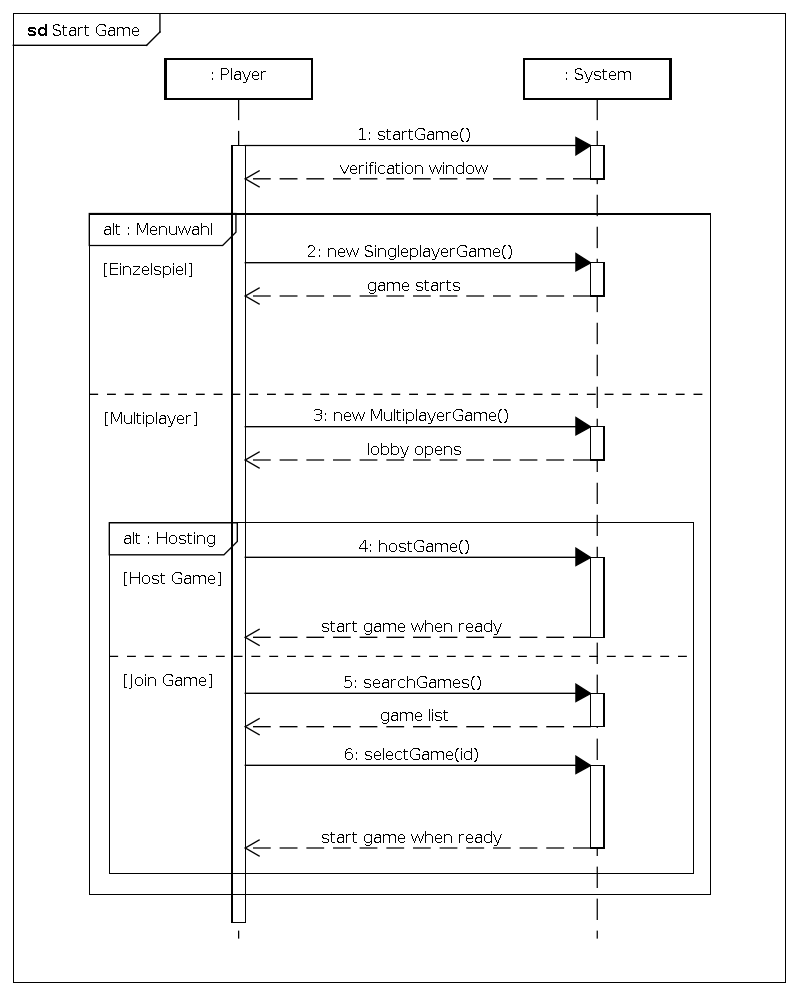
\includegraphics[width=0.85\textwidth]{SequenceDiagram.png}
 \end{center}
 \caption{Use Case UC1 ``Start Game'': Sequenzdiagramm}
 \label{fig:Sequenzdiagramm}
\end{figure}

%\subsection{Klassendiagramm}  (Müssen wir noch nicht machen)
 \newpage
\section{Systemoperationen}

Die folgenden Contracts beschreiben alle Systemoperationen des Use Cases UC1 ``Start Game'', welche im Sequenzdiagramm aufgeführt sind. Hierbei wird aufgezeigt, welche Operationen der User im Startprozess auslösen kann und was die Antwort des Systems darauf ist.

\subsection{Contract CO1: startGame}

\begin{tabular}{| p{0.2\textwidth} p{0.75\textwidth} |}
\hline
\textbf{Operation:} & \verb+void startGame()+ \\
\textbf{Querverweise:} & Use Cases: Start Game \\
\textbf{Vorbedingungen:} & - \\
\textbf{Nachbedingungen:} & \SquareShadowB \hspace{1mm} Das Spiel wurde gestartet \\
 & \SquareShadowB \hspace{1mm} Das Anmeldefenster ist erschienen\\
\hline
\end{tabular}

\subsection{Contract CO2: new SingleplayerGame}

\begin{tabular}{| p{0.2\textwidth} p{0.75\textwidth} |}
\hline
\textbf{Operation:} & \verb+new SingleplayerGame()+ \\
\textbf{Querverweise:} & Use Cases: Start Game \\
\textbf{Vorbedingungen:} & - Das Spiel wurde bereits gestartet\\
 & - Der Benutzer ist mit dem Server verbunden\\
\textbf{Nachbedingungen:} & \SquareShadowB \hspace{1mm} Ein Einzelspieler-Spiel wurde gestartet\\
\hline
\end{tabular}

\subsection{Contract CO3: new MultiplayerGame}

\begin{tabular}{| p{0.2\textwidth} p{0.75\textwidth} |}
\hline
\textbf{Operation:} & \verb+new MultiplayerGame()+ \\
\textbf{Querverweise:} & Use Cases: Start Game \\
\textbf{Vorbedingungen:} & - Das Spiel wurde bereits gestartet\\
 & - Der Benutzer ist mit dem Server verbunden\\
\textbf{Nachbedingungen:} & \SquareShadowB \hspace{1mm} Die Multiplayer Lobby wird angezeigt\\
\hline
\end{tabular}

\subsection{Contract CO4: hostGame}

\begin{tabular}{| p{0.2\textwidth} p{0.75\textwidth} |}
\hline
\textbf{Operation:} & \verb+void hostGame()+ \\
\textbf{Querverweise:} & Use Cases: Start Game \\
\textbf{Vorbedingungen:} & - Das Spiel wurde bereits gestartet\\
 & - Der Spieler hat den Multiplayer Modus gewählt\\
\textbf{Nachbedingungen:} & \SquareShadowB \hspace{1mm} Der Spieler hostet ein Spiel und wartet auf weitere Spieler\\
 & \SquareShadowB \hspace{1mm} Sind alle Spieler bereit, wird das Multiplayer Spiel gestartet\\
\hline
\end{tabular}

\subsection{Contract CO5: searchGame}

\begin{tabular}{| p{0.2\textwidth} p{0.75\textwidth} |}
\hline
\textbf{Operation:} & \verb+Game[] searchGame()+ \\
\textbf{Querverweise:} & Use Cases: Start Game \\
\textbf{Vorbedingungen:} & - Das Spiel wurde bereits gestartet\\
 & - Der Benutzer ist mit dem Server verbunden\\
 & - Der Spieler hat den Multiplayer Modus gewählt\\
\textbf{Nachbedingungen:} & \SquareShadowB \hspace{1mm} Es erscheint eine Liste mit den zur Zeit gehosteten Spieler, welche noch nicht gestartet sind.\\
\hline
\end{tabular}

\subsection{Contract CO6: selectGame}

\begin{tabular}{| p{0.2\textwidth} p{0.75\textwidth} |}
\hline
\textbf{Operation:} & \verb+Game selectGame(int id)+ \\
\textbf{Querverweise:} & Use Cases: Start Game \\
\textbf{Vorbedingungen:} & - Das Spiel wurde bereits gestartet\\
 & - Der Benutzer ist mit dem Server verbunden\\
 & - Der Spieler hat den Multiplayer Modus gewählt\\
 & - Der Spieler hat gewählt, dass er einem Spiel beitreten will\\
\textbf{Nachbedingungen:} & \SquareShadowB \hspace{1mm} Der Spieler hat ein Spiel gewählt und wartet auf weitere Spieler\\
 & \SquareShadowB \hspace{1mm} Sind alle Spieler bereit, wird das Multiplayer Spiel gestartet\\
\hline
\end{tabular}

 \newpage
\section{Architektur}

Das CCTD-Projekt ist Netzwerk-Applikation, welche aus zwei Hauptteilen besteht: Das effektive Spiel und eine Server-Komponente, welche die Lobby zur Verfügung stellt und alles andere, was für die Initialisierung eines Spieles nötig ist. Die Server-Komponente muss unabhängig von der Spiel-Komponente sein, damit Erweiterung am Server einen minimalen Einfluss auf das Spiel selber hat und damit in einem späteren Schritt dediziert gestart werden kann. Es handelt sich somit um einen Fat-Client. \\
Es ist im Allgemeinen angebracht, dass ein solches System auf dem Schichten-Model aufbauen sollte. Dies ist eine starke Unterstützung, um die Komplexität des System zu reduzieren und so minimal komplexen Programmcode zu erhalten. Moderne System werden in der Regel in 3 Schichten aufgeteilt: UserInterface, Domain, Logic.

\subsection{Logische Architektur}
\addcontentsline{lof}{figure}{Logische Architektur}
\begin{figure}[htb]
 \begin{center}
  \leavevmode
  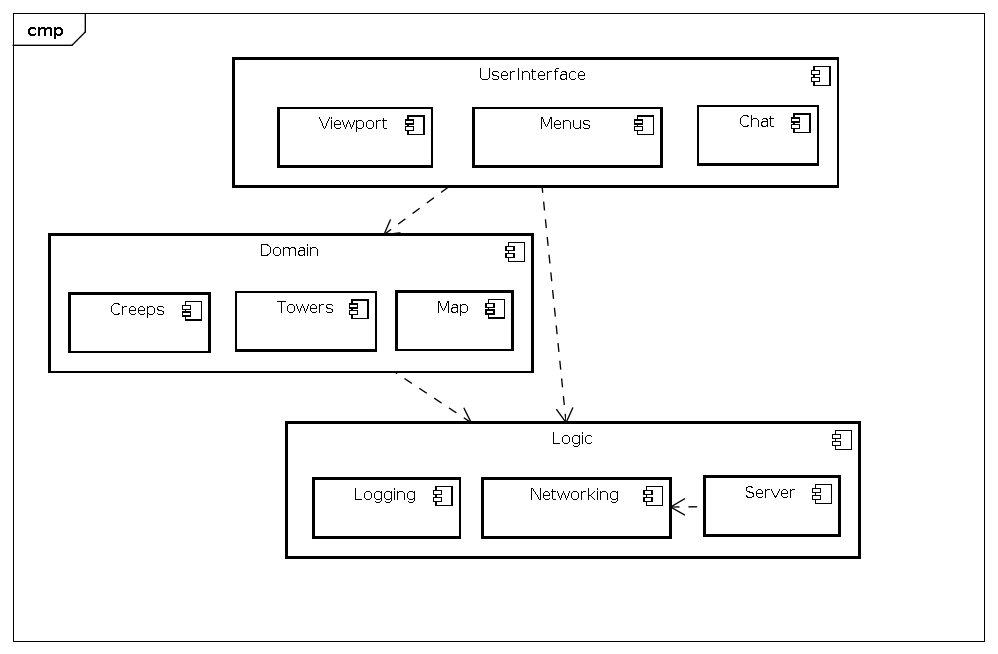
\includegraphics[width=0.95\textwidth]{logische_architektur.png}
 \end{center}
 \label{fig:logische_architektur}
\end{figure}
\addcontentsline{lot}{table}{Beschreibung: Logische Architektur}
\begin{longtable}{ | l | p{12cm} | }
 \hline
 \multicolumn{2}{|c|}{\textbf{UserInterface}} \\
 \hline
 \textbf{\glossary{name={Viewport}, description={Virtuelles Fenster für den Benutzer wodurch sie/er einen Bereich des Spiels sieht}}{Viewport}} & Zeichnet und definiert den sichtbaren Teil der Karte. \\
 \\
 \textbf{Menus} & Bietet Aktionen (Build,Upgrade,...) während dem Spiel an. \\
 \textbf{Chat} & UI-Elemente für den Spieler-Chat. \\
 \hline
 \multicolumn{2}{|c|}{\textbf{Domain}} \\
 \hline
 \textbf{\glossary{name={Creep}, description={gegnerisches Monster, welches abgeschossen werden soll}}{Creep}s} & Alle Arten von Creeps. \\
 \textbf{Towers} & Alle Arten von Towers inklusive ihren Upgrade Möglichkeiten. \\
 \textbf{Map} & Die Karte und alle Elemente, die sich direkt auf die Karte beziehen. \\
 \hline
 \multicolumn{2}{|c|}{\textbf{Logic}} \\
 \hline
 \textbf{Logging} & Bietet eine einheitliche Logging-Schnittstelle für die gesamte Applikation. \\
 \textbf{Networking} & Stellt eine Schnittstelle für die Kommunikation mit physikalisch entfernten Teil der Applikation zur Verfügung. \\
 \textbf{Server} & Beobachtet und Kontrolliert den Spielablauf, bietet eine Lobby \\
 \hline
\end{longtable}

 \newpage
\addcontentsline{toc}{section}{Glossar}
\printglossary \newpage
\addcontentsline{toc}{section}{Abbildungen}
\listoffigures
\addcontentsline{toc}{section}{Tabellen}
\listoftables

\end{document}
<\PRE>
